\chapter{Simulační výsledky}
V této kapitole ukážeme výsledky výpočtů Rényiho odhadů na námi generovaných datech. 



\section{Minimalizace}
Základem našich výpočtů je obecně vícerozměrná minimalizace funkcí definujících Rényiho vzdálenosti na různých rozděleních. O funkcích, které minimalizujeme obecně nevíme, zda jsou diferencovatelné, ani kolik mají lokálních minim. Radim Demut v \cite{Demut2010} používal pro výpočty metodu sítí, která je sice velmi spolehlivá, ale velmi pomalá. Hlavně kvůli zrychlení minimalizace jsme proto pracovali s klasickým algoritmem simulovaného žíhání. Typický stavový prostor, který bylo potřeba prohledávat je znázorněn na obrázcích \ref{fig-distanceL}, \ref{fig-distanceC}, \ref{fig-distanceE}. Ve svislé ose je vždy vynesena poloha $\mu$ a ve vodorovné je měřítko $\lambda$ pro Laplaceovo a exponenciální a $\sigma$ pro Cauchyovo rozdělení.

\begin{figure}[htb!]
	\begin{center}
		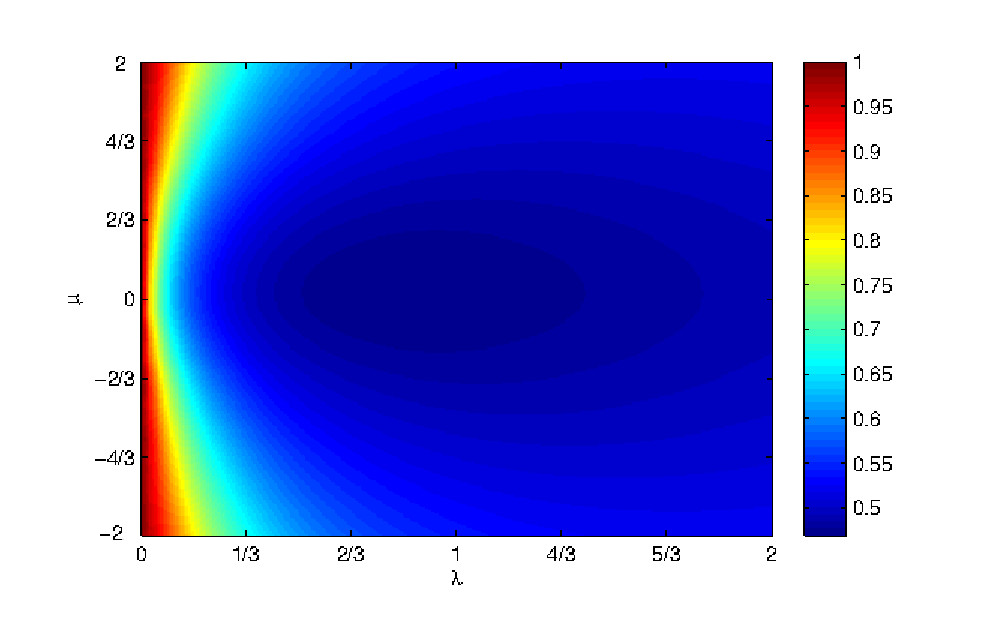
\epsfig{file=L01-L010-distance-e03-a03_mark2.eps, height=2.5in}
		\caption{Ukázka hodnot Rényiho pseudovzdálenosti s parametrem $\alpha = 0.3$. Zde jde o data generovaná jako konvexní směs Laplaceových distribucí $0.7\mathrm{L}(0,1) + 0.3 \mathrm{L}(0,10)$.}
		\label{fig-distanceL}
	\end{center}
\end{figure}

\begin{figure}[htb!]
	\begin{center}
		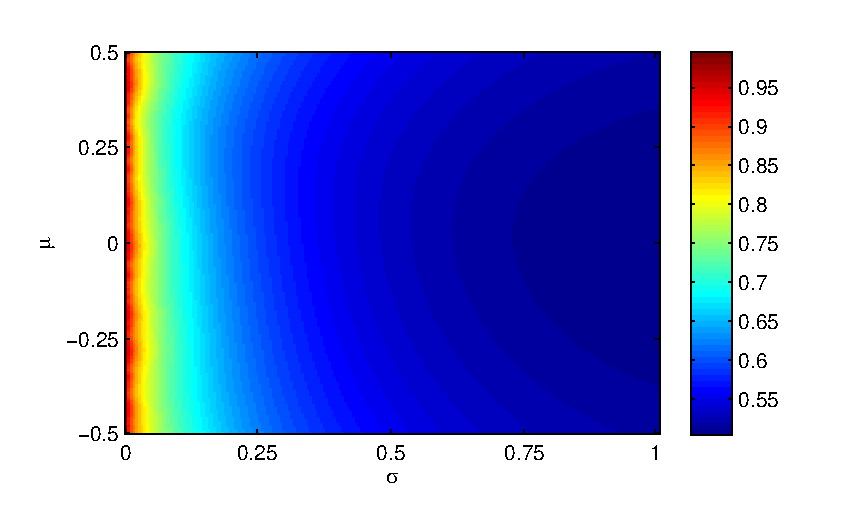
\epsfig{file=C01-err10x0.2-a05-dist.eps, height=2.5in}
		\caption{Ukázka hodnot Rényiho pseudovzdálenosti s parametrem $\alpha = 0.5$. Zde jde o data Z Cauchyho modelu s chybou $0.8\mathrm{C}(0,1) + 0.2 \mathrm{C}_{10}(0,1)$.}
		\label{fig-distanceC}
	\end{center}
\end{figure}

\noindent Sice jde jen o příklady, ale i pro jiná data vycházejí velmi podobné vizualizace. Obrázek \ref{fig-distanceC} je v poněkud větším detailu, takže je poněkud lépe vidět, že i tak nemá funkce nějaké nepříjemné lokální extrémy. Je tedy vidět, že minimalizovaná funkce je poměrně hladká a nejen, že není potřeba procházet celý stavový prostor pomocí metody sítí, ale dá se dokonce použít jednoduše modifikovaný "hill climber," který není zpomalovaný ani náhodným se vracením, které je tak důležité pro simulovaného žíhání. 

My jsme měli navíc zjednodušenou situaci tím, že jsme věděli, kde máme minimum hledat. 

Náš minimalizační algoritmus tedy vypadal následovně:
\vspace{11 pt}
\\
\textbf{Minimalizační algoritmus "hill climber"}

\begin{enumerate}
	\item Zvolíme dvourozměrný interval $[a_1,a_2]\times [b_1,b_2]$, ve kterém budeme hledat minimum funkce $f$.
	\item Zvolíme počáteční krok metody $\varepsilon$.
	\item Vyhodnotíme funkci v inicializačním bodě $x = (a,b),$ kde $a \in [a_1,a_2],\; b \in [b_1,b_2]$	
	\item Najdeme 8 bodů $\lbrace x_1,\ldots,x_8 \rbrace$ na rozích a uprostřed stran čtverce s délkou strany $2\varepsilon$ v jehož středu je bod $x$.	
	\item Pokud jsou body v námi prohledávané oblasti, najdeme $x_{\min} = \arg\min \lbrace f(x),f(x_1),\ldots,f(x_8)\rbrace$
		\begin{enumerate}
			\item Pokud je minima dosaženo v bodu $x_i \in \lbrace x_1,\ldots,x_8 \rbrace$, položíme $x := x_i$ a pokračujeme bodem 4.
			\item Pokud je v bodě $x$ stále funkční hodnota nejmenší položíme $\varepsilon:= \frac{\varepsilon}{2}$ a pokračujeme bodem 4.
		\end{enumerate}		
	\item 
	
	
\end{enumerate}

\begin{figure}[htb!]
	\begin{center}
		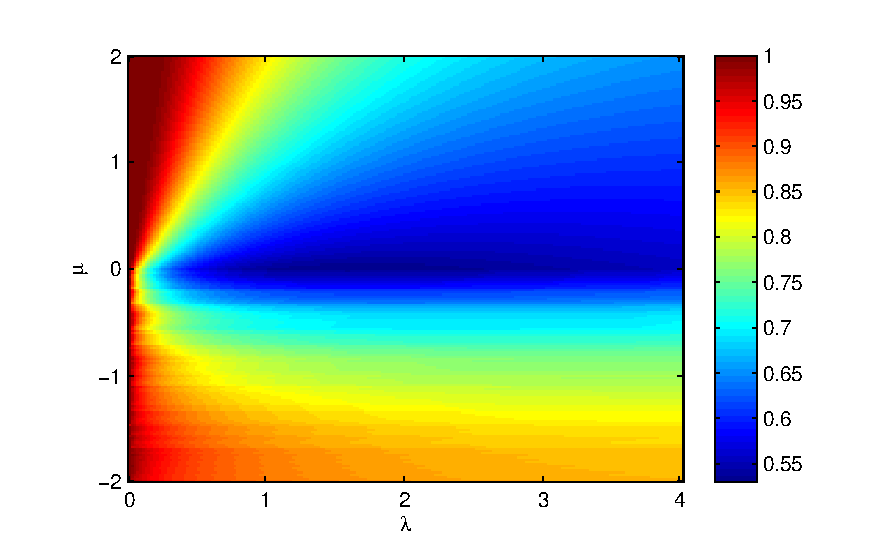
\epsfig{file=E01-E010-e04-a05-dist.eps, height=2.5in}
		\caption{Ukázka hodnot Rényiho pseudovzdálenosti s parametrem $\alpha = 0.5$. Data jsou generovaná jako konvexní směs exponenciálních rozdělení $0.6\mathrm{E}(0,1) + 0.4 \mathrm{E}(0,10)$.}
		\label{fig-distanceE}
	\end{center}
\end{figure}





Jelikož nám šlo o experimentální ověření robustnosti odhadů, generovali jsme znečištěná data v podobě konvexních směsí znečištěného rozdělení $P$ a znečišťujícího rozdělení $Q$, tedy směsi tvaru $P_\varepsilon(Q) = (1-\varepsilon)P + \varepsilon Q$, pro $\varepsilon \in [0,1]$. V tabulkách i grafech se objevuje 

\begin{figure}[htb]
	\begin{center}
		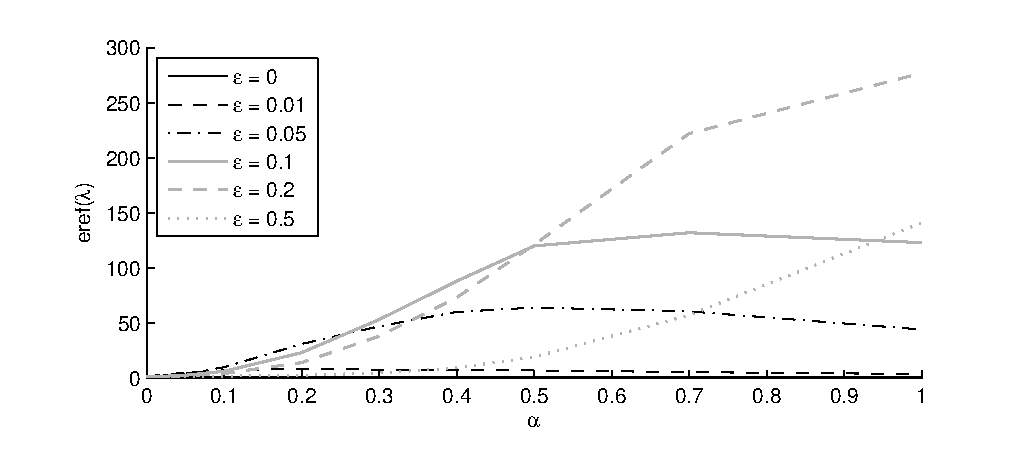
\epsfig{file=Eref-Exp-lambda.eps, height=2.in}
		\caption{Empirická relativní eficience eref($\hat{\lambda}$) minimálního $\mathfrak{R}_\alpha$-odhadu parametru $\lambda$ exponenciálního rozdělení v konvexní směsi 
		$(1-\varepsilon)E(0,1) + \varepsilon E(0,10)$ pro různá znečištění $\varepsilon$.}
		\label{fig-eref-Exp-lambda}
	\end{center}
\end{figure}

\begin{figure}[htb]
	\begin{center}
		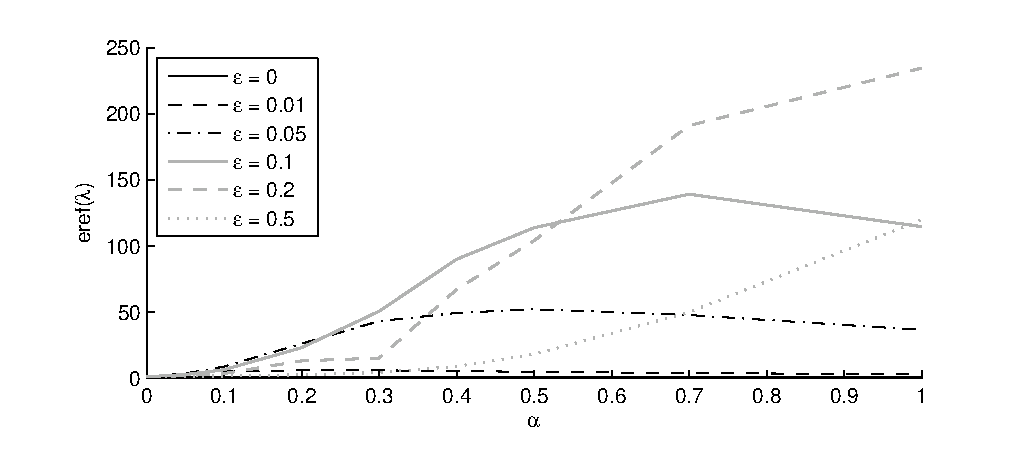
\epsfig{file=Eref-Laplace-lambda.eps, height=2.in}
		\caption{Empirická relativní eficience eref($\hat{\lambda}$) minimálního $\mathfrak{R}_\alpha$-odhadu parametrů  $\mu,\lambda$ Laplaceova rozdělení na datovém souboru o velikosti $n = 500$ generovaném	jako konvexní směs	$(1-\varepsilon)L(0,1) + \varepsilon L(0,10)$ pro různá znečištění $\varepsilon$.}
		\label{fig-eref-Laplace-lambda}
	\end{center}
\end{figure}

\begin{figure}[htb]
	\begin{center}
		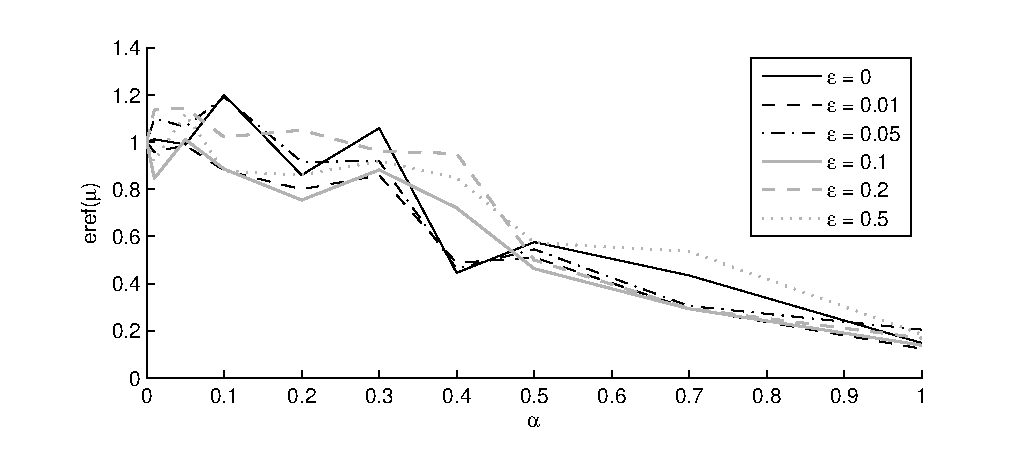
\epsfig{file=Eref-Exp-mu.eps, height=2.in}
		\caption{ TODO }
		\label{fig-eref-Exp-mu}
	\end{center}
\end{figure}

\begin{figure}[htb]
	\begin{center}
		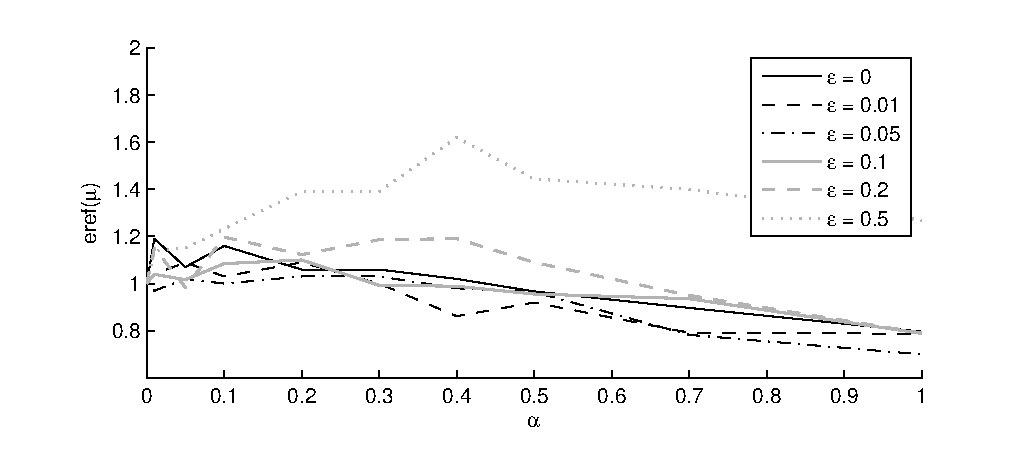
\epsfig{file=Eref-Laplace-mu.eps, height=2.in}
		\caption{ TODO }
		\label{fig-eref-Laplace-mu}
	\end{center}
\end{figure}

